\section{Introduction of $\BQP$}

\frame{
\frametitle{Introduction of $\BQP$}
\begin{block}{Definition of $\cclass{BQP}$}
\begin{itemize}
\item Informal: Class of efficiently solvable problems for full-fledged quantum computers
\pause
\item Formal: $\BQP$\ is the class of decision problems so that for each language $L\in\BQP$ there exists a polynomial-time \QTM\ $\Q_L$ that decides $L$:
\pause
\begin{align*}
    x\in L\Rightarrow \Pr{\Q_L(x)=1}\geq\frac{2}{3}
    \\
    x\notin L\Rightarrow \Pr{\Q_L(x)=0}\ge\frac{2}{3}
\end{align*}
\end{itemize}
\end{block}
}

\section{Relations of $\BQP$}

\frame{
\frametitle{Bounds on $\BQP$}
  \vfill
  \begin{beamercolorbox}[center]{title}
  How powerful are quantum computers?
  \end{beamercolorbox}
  \vfill
}

\subsection{$\BQP$\ vs $\P$}

\frame{
  \LARGE
\frametitle{$\BQP$\ vs $\P$}
  \vfill
  \begin{beamercolorbox}[center]{title}
  \only<2>{$\EXP$\ ?}
  \begin{equation*}
      \P\rightarrow\BQP
  \end{equation*}
  \end{beamercolorbox}
  \vfill
}

\subsection{$\BQP$\ vs $\EXP$}

\frame{
\frametitle{$\BQP$\ vs $\EXP$}
\begin{block}{Simulation Theorem}
For every \QTM\ $\Q$, given an input $x$, there exists an $\EXP$ TM $\M$ that calculates the probability amplitudes of the entire configuration graph of $\Q(x)$ with sufficient accuracy and thus decides $L_{\Q}$.
\pause
\\
Therefore $\BQP\subseteq\EXP$.
\end{block}
}

\frame{
\frametitle{$\BQP$\ vs $\EXP$}
\begin{block}{Definition of $\epsilon$-Closeness}
A \QTM\ $\Qdash$ is $\epsilon$-close to a \QTM\ $\Q$ \!\note{same alphabet and state set} iff the distance between each of their corresponding transition amplitudes is at most $\epsilon$.
\end{block}
}

\frame{
  \LARGE
\frametitle{$\BQP$\ vs $\EXP$}
  \vfill
  \begin{beamercolorbox}[center]{title}
  How close must $\Q$ and $\Qdash$ be for
  \begin{equation*}
    \exists c'>0:\forall x\in L_{\Q}:\Pr{\Qdash(x)=1}\geq\frac{1}{2}+c'
    \ ?
  \end{equation*}
  \end{beamercolorbox}
  \vfill
}

\frame{
\frametitle{$\BQP$\ vs $\EXP$}
\begin{block}{Discretization of $\cclass{BQP}$ QTMs}
\begin{itemize}
    \item $\Q$ and $\Qdash$ are $\epsilon$-close
    \pause
    \note{Combination of Theorem 3.7 and 3.9}
    \item $\Rightarrow\norm{\ket{\phi'_{p(n)}}-\mathrm{U}^{p(n)}\ket{\phi_0}}\leq 2\cdot\vert\Sigma\vert\cdot\vert Q\vert\cdot\epsilon\cdot p(n)\pause =:\delta$
    \pause
    \note{Theorem 3.6}
    \item $\Rightarrow\forall x\in L:\Pr{\Qdash_L(x)=1}\geq\underbrace{\Pr{\Q_L(x)=1}}_{\frac{1}{2}+c}-4\delta$
    \pause
    \item Logarithmic many bits in precision of amplitudes are sufficient for $\Qdash$ to be a $\BQP$ machine
\end{itemize}
\end{block}
}

\frame{
\frametitle{$\BQP$\ vs $\EXP$}
\vfill
  \begin{beamercolorbox}[center]{title}
  Configuration graph of $\Qdash(x)$
    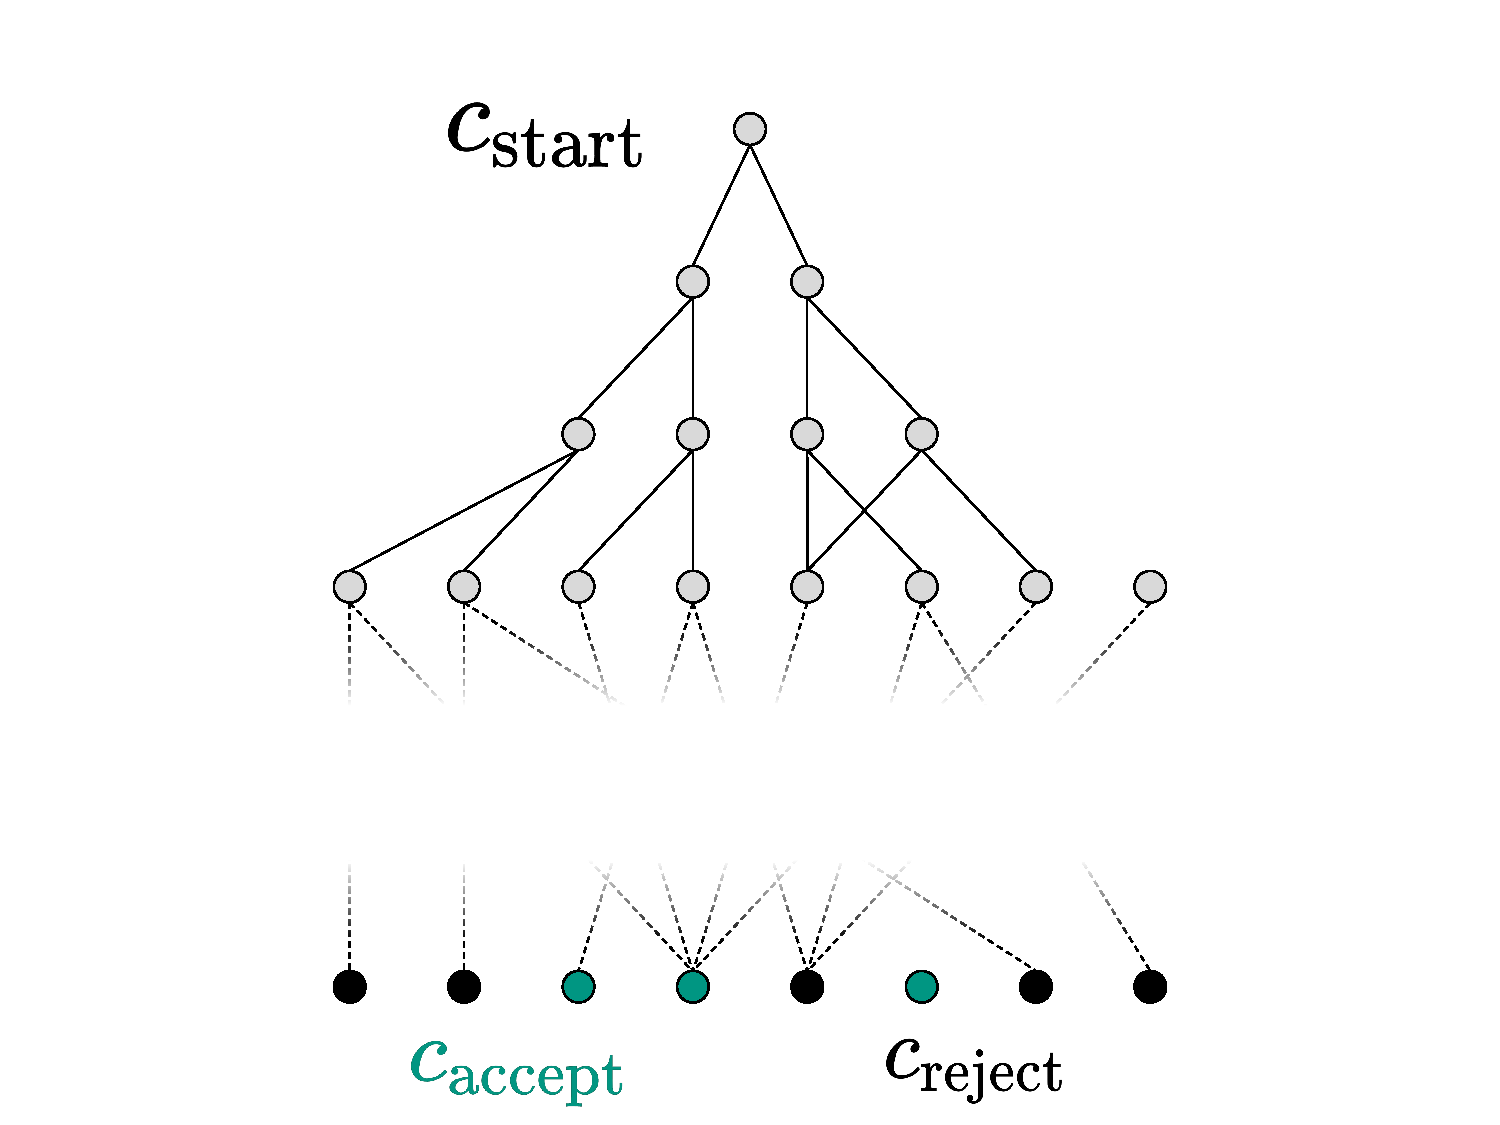
\includegraphics[width=0.8\textwidth,keepaspectratio]{images/ConfigurationGraph}
  \end{beamercolorbox}
\vfill
}

\frame{
  \LARGE
\frametitle{$\BQP$\ vs $\P$}
\vfill
  \begin{beamercolorbox}[center]{title}
  \only<2>{$\PSPACE$\ ?}
  \begin{equation*}
      \P\rightarrow\BQP\rightarrow\EXP
  \end{equation*}
  \end{beamercolorbox}
  \vfill
}

\subsection{$\BQP$\ vs $\PSPACE$}

\frame{
\frametitle{$\BQP$\ vs \textcolor{gray}{\sout{$\EXP$}} $\PSPACE$}
\vfill
\begin{columns}
\begin{column}{.5\textwidth}
    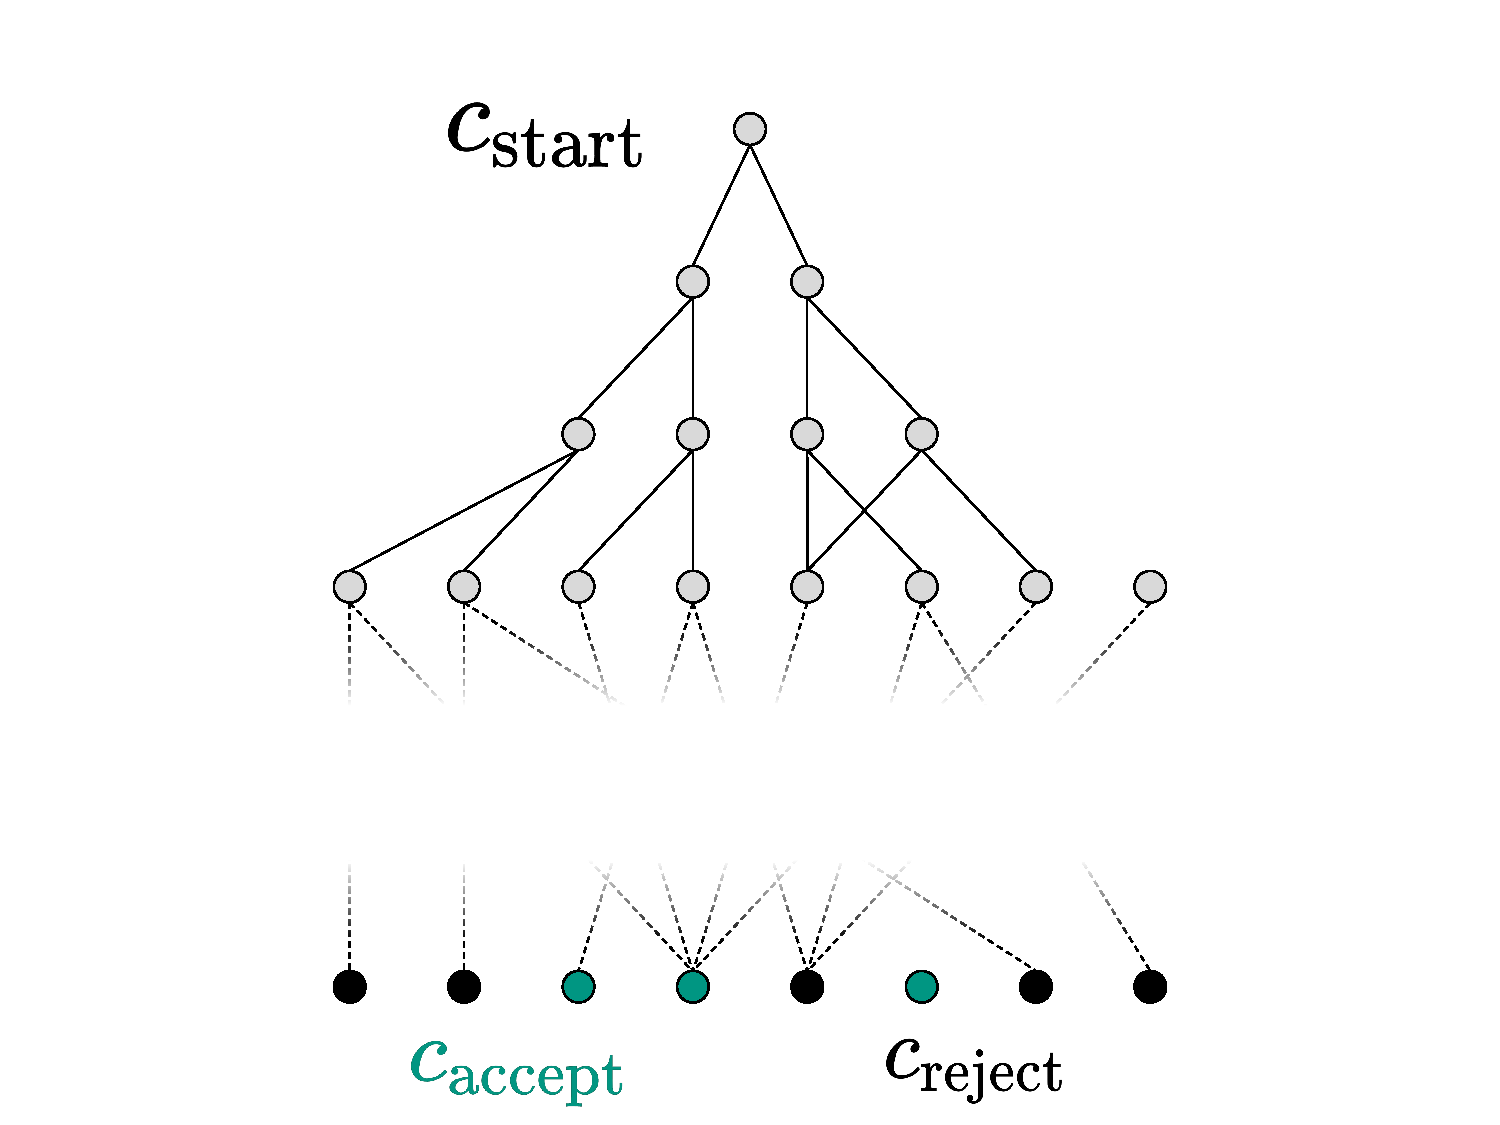
\includegraphics[width=1.5\textwidth,keepaspectratio]{images/ConfigurationGraph}
\end{column}
\begin{column}{.1\textwidth}
    \hspace*{.75cm}
    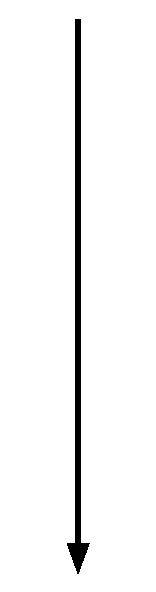
\includegraphics[width=\textwidth,keepaspectratio]{images/ArrowDown}
\end{column}
\pause
\begin{column}{.4\textwidth}
\centering
max path length
\\
at most $p(n)$
\\
\pause
$\Rightarrow$ DFS
\end{column}
\end{columns}
\vfill
}

\frame{
  \LARGE
\frametitle{$\BQP$\ vs $\PSPACE$}
\vfill
  \begin{beamercolorbox}[center]{title}
  \only<2>{$\BPP$\ ?}
  \begin{equation*}
      \P\rightarrow\BQP\rightarrow\PSPACE\rightarrow\EXP
  \end{equation*}
  \end{beamercolorbox}
  \vfill
}

\subsection{$\BQP$\ vs $\BPP$}

\frame{
\frametitle{$\BQP$\ vs $\BPP$}
\begin{block}{Bounded-Error Polynomial-Time}
\begin{itemize}
\item $\BQP$ is the quantum generalization of $\BPP$.
\pause
\item Every PTM $\M_L$ is canonically extendable to a \QTM\ $\Q_L$ with the same runtime and the same output as $\M_L$ for every $x\in L$\pause, thus $\BPP\subseteq\BQP$.
\end{itemize}
\end{block}
}

\frame{
  \LARGE
\frametitle{$\BQP$\ vs $\BPP$}
  \begin{beamercolorbox}[center]{title}
  \begin{equation*}
      \BPP\overset{?}{=}\BQP
  \end{equation*}
  \end{beamercolorbox}
\pause
\Large
\begin{columns}
\begin{column}{.5\textwidth}
  \begin{equation*}
  \begin{array}{rrcl}
      &\BPP\!&\neq&\!\BQP
      \\
      \Leftrightarrow&
      \BPP&\subset&\BQP
      \\
      \Rightarrow&
      \P&\overset{!}{\subset}&\PSPACE
  \end{array}
  \end{equation*}
\end{column}
\pause
\hspace*{-1cm}\vrule
\begin{column}{.5\textwidth}
  \begin{equation*}
  \begin{array}{rrcl}
      &\BPP&=&\BQP
      \\
      \Rightarrow&
      \P&\overset{?}{=}&\PSPACE
  \end{array}
  \end{equation*}
\end{column}
\end{columns}
  \vfill
}

\frame{
  \LARGE
\frametitle{$\BQP$\ vs $\BPP$}
\vfill
  \begin{beamercolorbox}[center]{title}
  \only<2>{$\NP$\ ?}
  \begin{equation*}
      \P\rightarrow\BPP\rightarrow\BQP\rightarrow\PSPACE\rightarrow\EXP
  \end{equation*}
  \end{beamercolorbox}
  \vfill
}

\subsection{$\BQP$\ vs $\NP$\ and $\NPC$}

\frame{
  \LARGE
\frametitle{$\BQP$\ vs $\NP$ and $\NPC$}
\vfill
  \begin{beamercolorbox}[center]{title}
  \begin{equation*}
      \P\rightarrow\BPP
      \begin{array}{c}
      \nearrow
      \\
      \searrow
      \end{array}
      \begin{array}{c}
      \BQP
      \\
      \only<2>{\uparrow\downarrow ?}
      \\
      \NP
      \end{array}
      \begin{array}{c}
      \searrow
      \\
      \nearrow
      \end{array}
      \PSPACE\rightarrow\EXP
  \end{equation*}
  \end{beamercolorbox}
  \vfill
}

\frame{
\frametitle{$\BQP$\ vs $\NP$ and $\NPC$}
\Large
\begin{block}{Conjecture}
\centering
\vspace*{1em}
  $\BQP\cap\NPC=\emptyset$
\vspace*{1em}
\end{block}
}

\frame{
\frametitle{$\BQP$\ vs $\NP$ and $\NPC$}
\begin{block}{Conjecture: $\cclass{BQP}\cap\NPC=\emptyset$}
\begin{itemize}
\item $\NPI:=\NP\setminus(\P\cup\NPC)$
\pause
\item $\P\neq\NP\Leftrightarrow\NPI\neq\emptyset$ (Ladner's theorem)
\pause
\item $\text{Shor's algorithm}\Rightarrow\mathit{IF}\in\BQP$
\pause
\item $IF\in\NPI\Rightarrow\BQP\not\subseteq\NPC$
\pause
\item Counterargument: $\BQP\subseteq\NPC\Rightarrow\P=\NP$ (unlikely)
\end{itemize}
\end{block}
}

\frame{
\frametitle{$\BQP$\ vs $\NP$ and $\NPC$}
\begin{block}{Conjecture: $\cclass{BQP}\cap\NPC=\emptyset$}
\begin{itemize}
\item What about $\NPC\subseteq\BQP$?
\pause
\item No quantum poly-time algorithm known (yet)
\pause
\item $\NPC\not\subseteq\BQP\Rightarrow\P\neq\NP$
\pause
\item $\rightarrow\NPC\not\subseteq\BQP$ conjectured ($\Rightarrow\NP\not\subseteq\BQP$)
\pause
\item $\NPC\not\subseteq\BQP$ and all $\NPC$ problems are equally hard
$\Rightarrow\BQP\cap\NPC=\emptyset$
\end{itemize}
\end{block}
}

\frame{
\frametitle{$\BQP$\ vs $\NP$ and $\NPC$}
\Large
  \begin{beamercolorbox}[center]{title}
  \begin{equation*}
      \BQP\overset{?}{\not\subseteq}\NP
  \end{equation*}
  \end{beamercolorbox}
\begin{columns}
\begin{column}{.5\textwidth}
  \begin{equation*}
  \BQP\subset\NP
  \end{equation*}
  \visible<2-3>{
  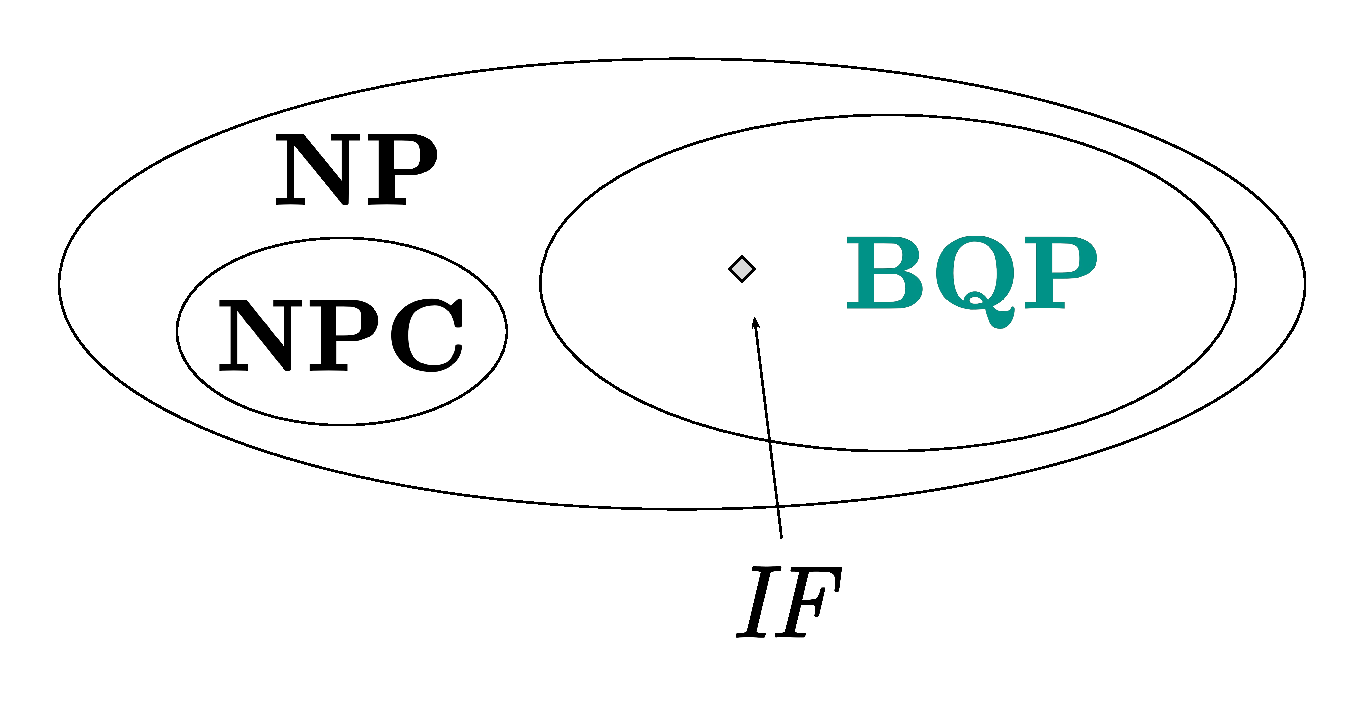
\includegraphics[width=\textwidth,keepaspectratio]{images/BQPsubsetNP}
  }
\end{column}
\hspace*{-1cm}\vrule
\begin{column}{.5\textwidth}
  \begin{equation*}
  \BQP\not\subseteq\NP
  \end{equation*}
  \visible<3>{
  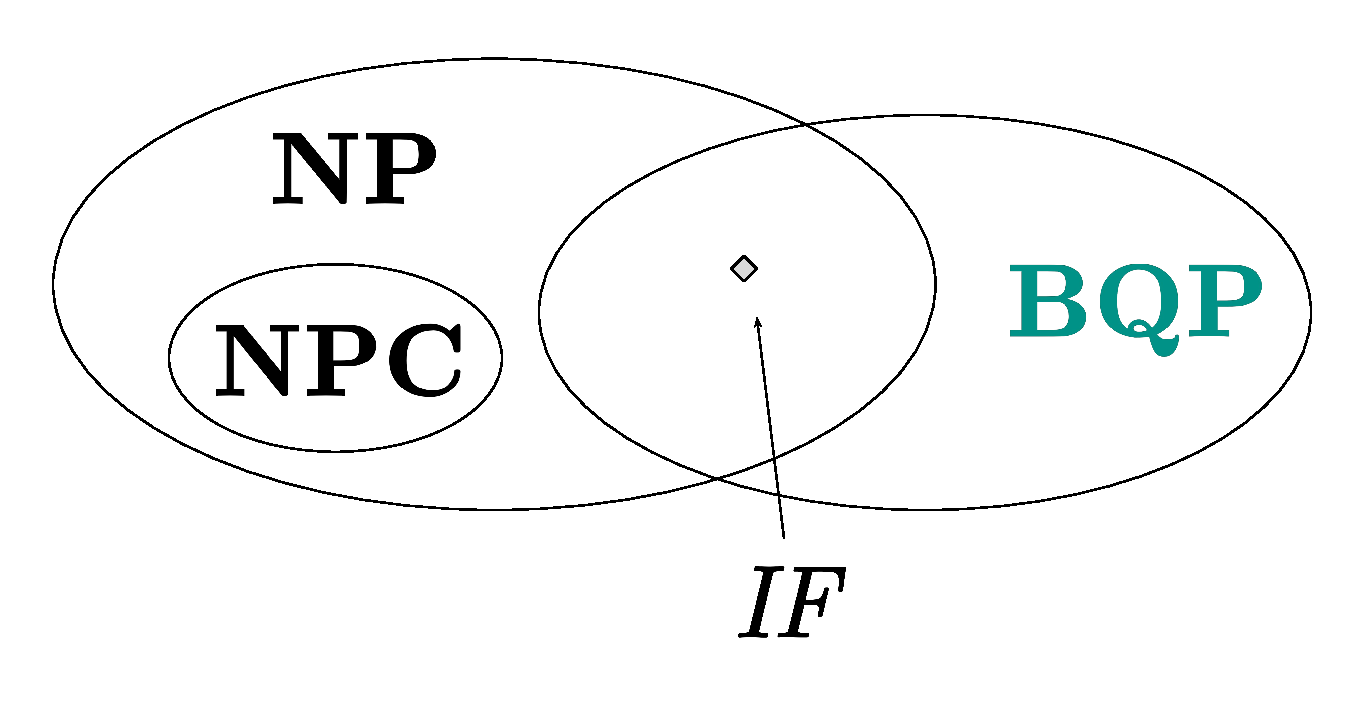
\includegraphics[width=\textwidth,keepaspectratio]{images/BQPnotsubsetNP}
  }
\end{column}
\end{columns}
  \vfill
}

\frame{
\Large
\frametitle{$\BQP$\ vs $\NP$ and $\NPC$}
\centering
  \begin{beamercolorbox}[center]{title}
  \begin{equation*}
      \BQP\not\subseteq\PH
      \Rightarrow
      \BQP\not\subseteq\NP
  \end{equation*}
  \end{beamercolorbox}
  \visible<2>{
  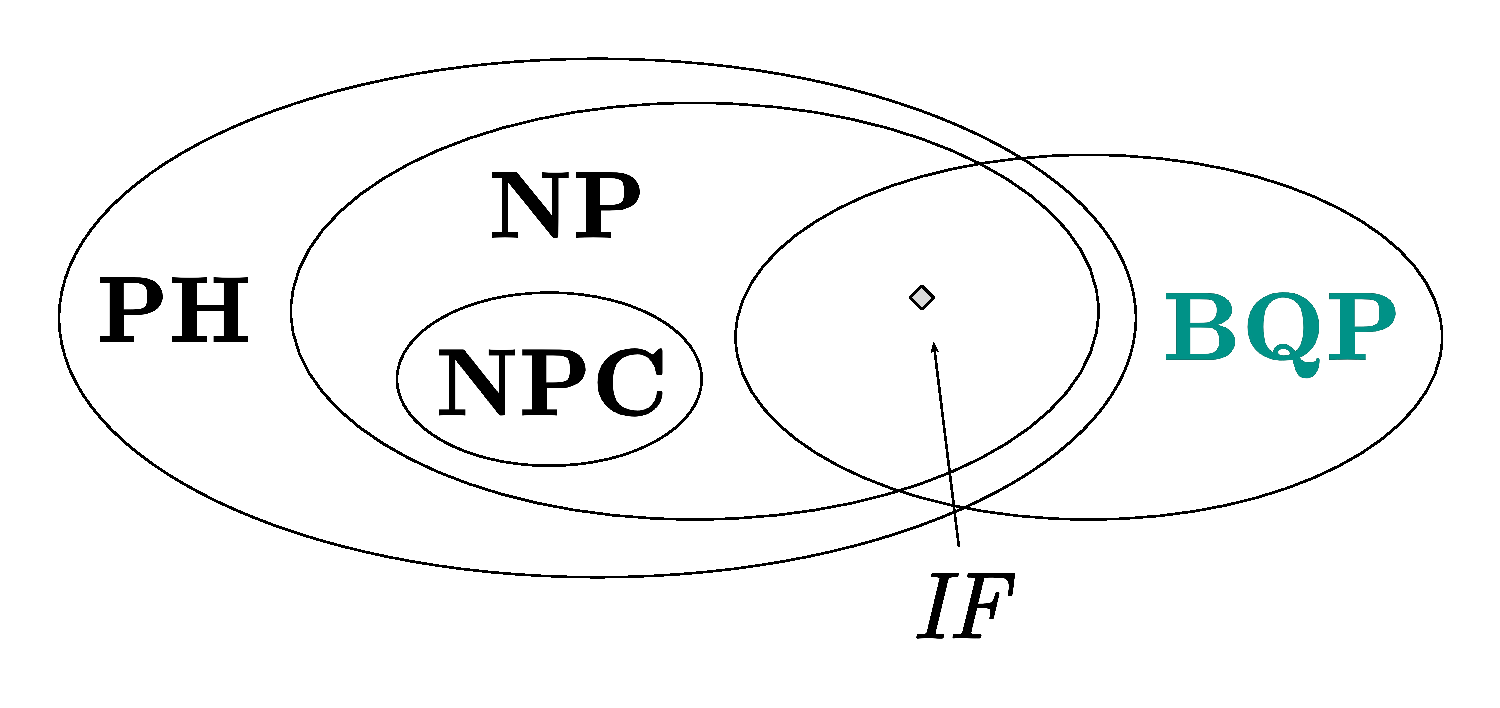
\includegraphics[width=.75\textwidth,keepaspectratio]{images/BQPnotsubsetPH}
  }
  \vfill
}

\section{Summary}

\frame{
\frametitle{Summary}
\centering
  \vfill
  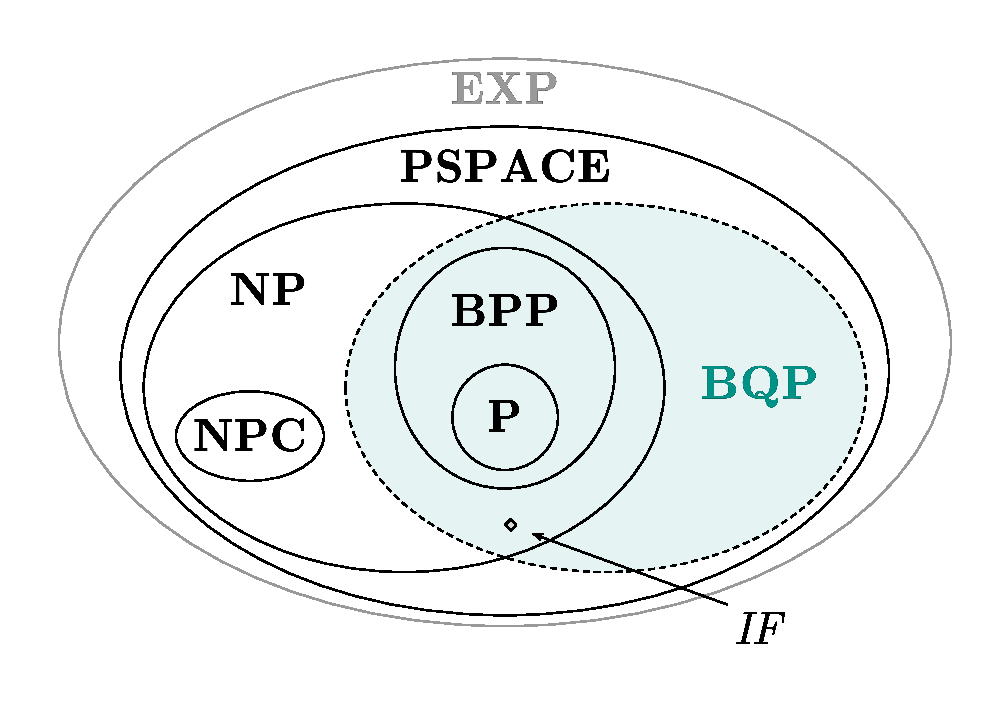
\includegraphics[width=\textwidth,keepaspectratio]{images/ContextofBQP}
  \vfill
}

\frame{
\frametitle{Summary}
\begin{block}{Results}
\begin{itemize}
\item Quantum computer at least as powerful as classical computers
\pause
\item Assumed: Superpolynomial speedup for problems outside $\NP$ and even $\PH$
\pause
\item Assumed: At most polynomial speedup for $\NPC$ problems
\pause
\item Theoretical results!
\end{itemize}
\end{block}
}

\frame{
\frametitle{References}
\vfill
\scriptsize
\begin{itemize}
\setlength\itemsep{.5em}
\item[{[1]}] Feynman, R. P. (1982). Simulating physics with computers. International Journal of Theoretical Physics,21(6-7), 467-488. doi:10.1007/bf02650179


\item[{[2]}] Grover, L. K. (1996). A fast quantum mechanical algorithm for database search. Proceedings of the Twenty-eighth Annual ACM Symposium on Theory of Computing - STOC 96. doi:10.1145/237814.237866


\item[{[3]}] Shor, P. W. (1997). Polynomial-Time Algorithms for Prime Factorization and Discrete Logarithms on a Quantum Computer. SIAM Journal on Computing, 26(5), 1484-1509. doi:10.1137/s0097539795293172


\item[{[4]}] Ladner, R. E. (1975). On the Structure of Polynomial Time Reducibility. Journal of the ACM, 22(1), 155-171. doi:10.1145/321864.321877


\item[{[5]}] Aaronson, S. (2010). BQP and the polynomial hierarchy. Proceedings of the 42nd ACM Symposium on Theory of Computing - STOC 10. doi:10.1145/1806689.1806711


\item[{[6]}] Bennett, C. H., Bernstein, E., Brassard, G., \& Vazirani, U. (1997). Strengths and Weaknesses of Quantum Computing. SIAM Journal on Computing, 26(5), 1510-1523. doi:10.1137/s0097539796300933
\end{itemize}
\vfill
}